\documentclass{article}
\usepackage{ctex}

% Set page size and margins
% Replace `letterpaper' with `a4paper' for UK/EU standard size
\usepackage[letterpaper,top=2cm,bottom=2cm,left=2.5cm,right=2.5cm,marginparwidth=1.75cm]{geometry}

% Useful packages
\usepackage{amsmath}
\usepackage{graphicx}
\usepackage{float}
\usepackage[colorlinks=true, allcolors=blue]{hyperref}

\title{微分方程数值解计算实习课后作业5}
\author{陈文宇}
\date{\today}


\begin{document}


\maketitle

\tableofcontents

\newpage
%---------------------------------------------------
\section{问题重述}

\begin{itemize}
    \item 画出数值解的图像
    \item 获取两类误差:
    $$ errL=(\int^{1}_{0}(\mu_{*}(x)-\mu_{n}(x))^{2}dx)^{\frac{1}{2}}$$
    $$ errH=(\int^{1}_{0}(\mu_{*}(x)-\mu_{n}(x))^{2}+(\mu'_{*}(x)-\mu'_{n}(x))^{2}dx)^{\frac{1}{2}}$$
    计算其关于网格长度的数值收敛阶
    \item 用$loglog()$函数展示$errL,errH,condA$的图像,
\end{itemize}
 
%---------------------------------------------------
\section{实验思路}
一维二次Lagrange型有限元方法求解:练习$2.1.1$
\[
\left\{
\begin{aligned}
	&-\mu '' + \frac{\pi^{2}}{4}\mu = \frac{\pi^{2}}{2}\sin{\frac{\pi}{2}x} \quad0<x<1 
	\\
	&\mu(0)=0 ,\quad \mu'(1)=0 
\end{aligned}
\right.
\]
对每个整结点和半结点构造基函数如下:对于i=1 2 ... n-1
\[
\phi_{i}(x)=
\left\{
\begin{aligned}
	&(2\frac{|x-x_{i}|}{h_{i}}-1)((\frac{|x-x_{i}|}{h_{i}}-1)   &x_{i-1}<x<x_{i}
	\\
	&(2\frac{|x-x_{i}|}{h_{i+1}}-1)((\frac{|x-x_{i}|}{h_{i+1}}-1) & x_{i}<x<x_{i+1}
        \\
        & \quad 0 & \text{其他}
\end{aligned}
\right.
\]

\[
\phi_{i+\frac{1}{2}}(x)=
\left\{
\begin{aligned}
	&4\frac{|x-x_{i}|}{h_{i+1}}(1-\frac{|x-x_{i}|}{h_{i+1}})   &x_{i}<x<x_{i+1}
	\\
        & \quad 0 & \text{其他}
\end{aligned}
\right.
\]

考虑试探函数空间$U_{n}=\{\phi_{i}\}_{i=1}^{n}$,对任意$u_{h}\in U_{h}$可以表示为:
$$u_{n}=\sum_{i=1}^{n}u_{i}\phi _{i}(x)+u_{i+\frac{1}{2}}\phi_{i+\frac{1}{2}(x)$$

形成有限元方程后,对其本质边界条件做处理,以求解线性方程组$Ax=b$即可获得基函数系数。
对于条件数可以使用matlab命令$cond(A,2)$,
定义errL和errH后,给出其在$ I_{i}$区间Guass结点的函数值,然后可以使用三点Guass求积公式来求积分,
进而使用$plot,loglog$函数绘制图像即可。

matlab编程的具体操作详见FEM\_1D2P\_L.m,在代码结构上采用了实习课老师分享的代码。
对于刚度矩阵,代码中仍旧先生成单元刚度矩阵,再扩建为整个刚度矩阵。


\newpage
%---------------------------------------------------
\section{实验结果}

下图是数值解和精确解的图像:
\begin{figure}[H]
\centering
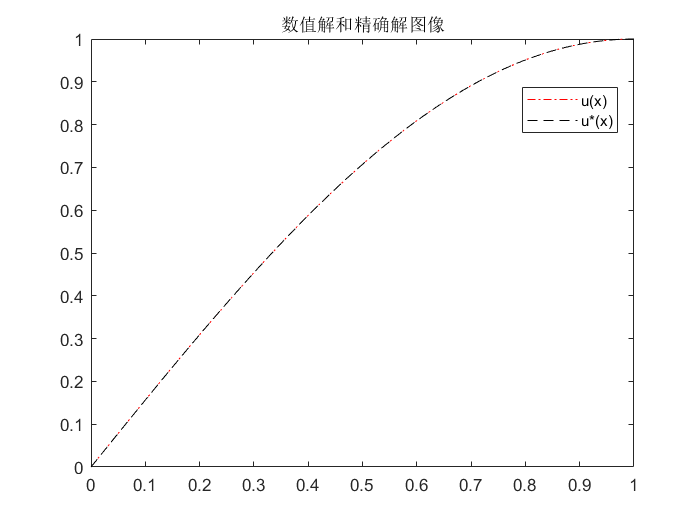
\includegraphics[scale=0.6]{solution_image.png}
\caption{\label{solution_image}数值解和精确解的图像}
\end{figure}

下图是$(logh,log(errL))$的图像,同$y=h^2$对比知,$errL$收敛阶为2.
\begin{figure}[H]
\centering
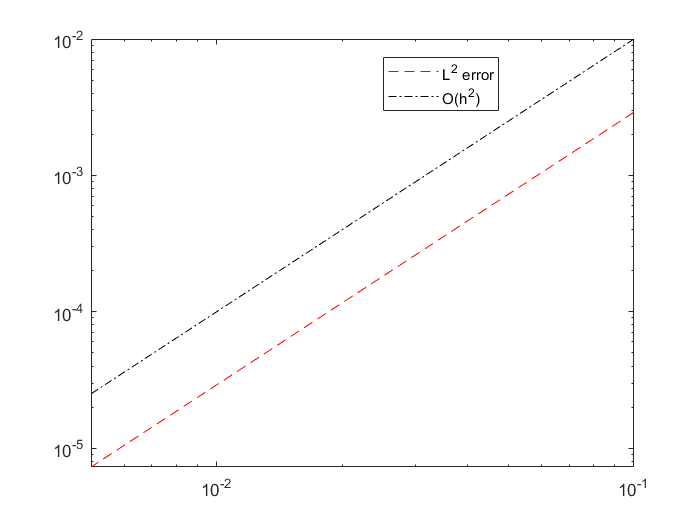
\includegraphics[scale=0.6]{L_err.png}
\caption{\label{L_err}$L^{2}([0,1])$误差的收敛阶}
\end{figure}


下图是$(logh,log(errH))$的图像,根据线性基本拟合,知$errH$收敛阶为2.
\begin{figure}[H]
\centering
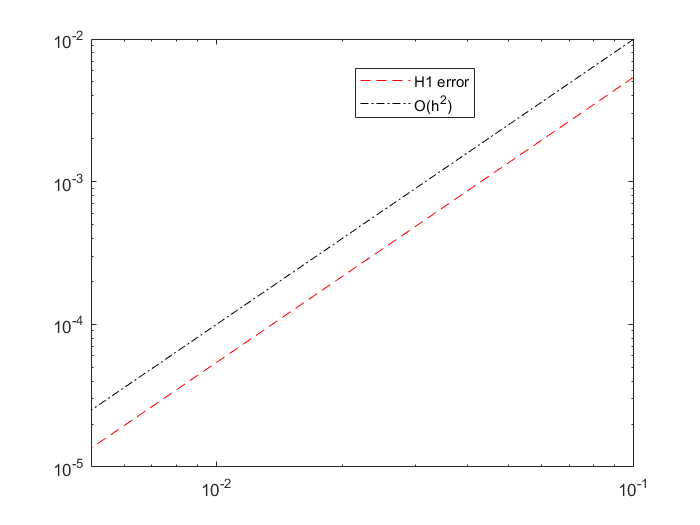
\includegraphics[scale=0.6]{H1_err.png}
\caption{\label{H1_err}$H^{1}([0,1])$误差的收敛阶}
\end{figure}



用$loglog()$函数展示矩阵A的条件数的变化。
\begin{figure}[H]
\centering
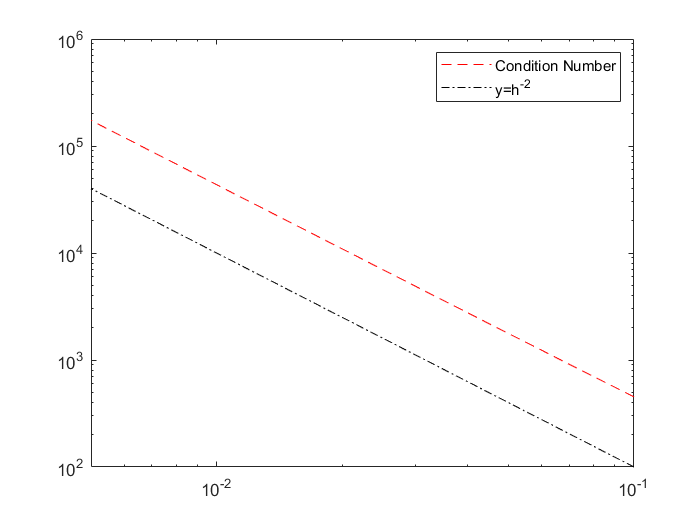
\includegraphics[scale=0.6]{CondA.png}
\caption{\label{CondA}$CondA$}
\end{figure}


%-----------------------------------------------------
\section{实验结果分析}
对于本题,两类误差的收敛阶均为2,矩阵A条件数有以下性质 $CondA$与同$h$成指数关系,且与$h^{-2}$同阶。
同一次有限元法做对比,errL的收敛阶从1变为2,收敛速度加快。

(二次有限元法已完成,三次有限元法程序编写存在问题,目前无法做出描述)

\end{document}